\documentclass[]{article}
\usepackage{caption,subcaption,graphicx,float,url,amsmath,amssymb,tocloft,wasysym,amsthm,thmtools,textcomp,listings,amsfonts,cancel}
\usepackage[hidelinks]{hyperref}
\usepackage[toc,acronym,nonumberlist]{glossaries}
\usepackage[]{algorithm2e}
\setacronymstyle{long-short}
\usepackage{glossaries-extra}
\graphicspath{{figs/}} 
\setlength{\cftsubsecindent}{0em}
\setlength{\cftsecnumwidth}{3em}
\setlength{\cftsubsecnumwidth}{3em}
\newcommand\numberthis{\addtocounter{equation}{1}\tag{\theequation}}
\newtheorem{thm}{Theorem}
\newtheorem{cor}[thm]{Corollary}
\setcounter{tocdepth}{1}

%opening
\title{Computation in Complex Systems\\
	Week 4\\Worst-case, Natural, and Random
	}


\begin{document}

\maketitle

\section{Phase Transitions}

\begin{enumerate}
	\item Referring to the Ising Model interactive in this unit:
	\begin{enumerate}
		\item What is the critical temperature ($\pm0.1$)?
		\item  Describe the relationship between spin correlation and lattice length (L/2) at the critical point. (No equations needed, simply provide a phrase describing the general relationship.)
	\end{enumerate}
	
	\item 	Referring to the Percolation interactive in this unit:
	\begin{enumerate}
		\item What is the critical site occupancy probability p ($\pm0.02$ )?
		
		\item Describe the relationship of non-giant component sizes and their frequency at the critical point.
	\end{enumerate}
\end{enumerate}


\section{Landscapes, Clustering, Freezing and Hardness}

Based on the plot below--Figure \ref{fig:content_SATalpha}--showing percent satisfiability (SAT) relative to $\alpha$ for two different N:

\begin{enumerate}
	\item  Generally speaking, what happens in the solvability space of SAT problems?

	\item  What does the vertical red dashed line indicate?

	\item   Where do you expect the computational time would be largest along the $\alpha$ axis?

	\item   BONUS*) Is the SAT party problem above satisfiable?
\end{enumerate}


\begin{figure}[H]
	\begin{center}
		\caption{percent satisfiability (SAT) relative to $\alpha$ for two different N}\label{fig:content_SATalpha}
		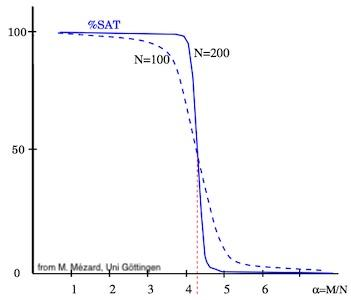
\includegraphics[width=0.6\textwidth]{content_SATalpha}
	\end{center}
\end{figure}
% bibliography go here

\bibliographystyle{unsrt}
\raggedright
\addcontentsline{toc}{section}{Bibliography}
\bibliography{computations}

\end{document}
